\chapter{Lecture 4}

%--- 信息 ----
\begin{center}
    讲师:王立威 \qquad
    课程时间:25.Mar.11th \qquad 
    笔记:25.June.7th
\end{center}

\bigskip

接着上节课的内容,根据上节课的两个定理可以得到:
\[
H(Y) \ge H(Y|X), \qquad H(X) \ge H(X|Y)
\]

这说明原有的信息量永远不小于条件下的信息量.这称作"Conditioning reduces entropy.",可以认为这是因为加上条件等价于在某种程度上引入了信息,从而降低了“新”的信息量. 

事实上,我们能推出 
\[
H(X) - H(X|Y) = H(Y) - H(Y|X) = H(X) + H(Y) - H(X,Y)
\]

据此引出新的定义 
\begin{definition}[互信息]
    对于两个随机变量$X,Y$,定义其\textbf{互信息}(mutual information)为 
    \[
    I(X;Y) := H(X) - H(X|Y) = H(X) + H(Y) - H(X,Y)
    \]
\end{definition}

互信息是可以用联合概率分布列表示的,表示法如下(请自行验证):
\[
I(X; Y) = \sum_{i,j} \Pr[X=x_i, Y=y_j] \log_2 \dfrac{\Pr[X=x_i, Y=y_j]}{\Pr[X=x_i]\cdot \Pr[ Y=y_j]}
\]

自然地,可类似定义任意多元随机变量$\boldsymbol{X}=(X_i)_{i=1}^n$的联合熵$H(\boldsymbol{X})$;也可定义两组随机变量$\boldsymbol{X}=(X_i)_{i=1}^n, \boldsymbol{Y}=(Y_j)_{j=1}^m$的条件熵$H(\boldsymbol{X}|\boldsymbol{Y})$和互信息$I(\boldsymbol{X};\boldsymbol{Y})$. 

\begin{theorem}
    对于多元随机变量$\boldsymbol{X}=(X_i)_{i=1}^n$,有 
    \[
    H(\boldsymbol{X}) = H(X_1) + H(X_2|X_1) + H(X_3|X_1,X_2) + \cdots + H(X_n|X_{1\sim (n-1)})
    \]
\end{theorem}

至此的讨论都基于随机变量$X$的分布列$P$是已知的,但在真实世界中我们往往无法精确观测或获取真实分布列.但取而代之,我们往往有一个估计(近似)$Q = (q_1,\dots, q_n)$,此时我们依照这个分布列编码,码长应为$(\log 1/q_1,\dots, \log 1/q_n)$,那么平均码长为 $\sum_{i=1}^n p_i \log 1/q_i$. 相较与最短码长$H(P)$,这样的编码存在冗余$\sum_{i=1}^n p_i \log p_i/q_i$,这就是著名的K-L散度. 

\begin{definition}[Kullback-Leibler 散度]
    对于两个分布列$P=(p_1,\dots, p_n)$和$Q=(q_1,\dots, q_n)$,其\textbf{Kullback-Leibler 散度}(divergence)定义为 
    \[
    D(P \| Q) := \sum_{i=1}^n p_i \log_2 \dfrac{p_i}{q_i}
    \]

    Kullback-Leibler 散度也称作K-L散度或相对熵(relative entropy).并且也可记作$\text{KL}(P\| Q)$.
\end{definition}

某种意义而言,K-L散度是比信息熵更加基础和重要的概念.在以后的例子中,我们会发现在有些情况下难以定义信息熵,但却可以定义K-L散度. 

另外,请注意K-L散度不是对称的,故不是距离度量.

\begin{example}[K-L散度的凸性]
    考虑以下情况:固定$Q$,$D$对$P$是凸的吗?固定$P$,$D$对$Q$是凸的吗?$D$对$(P, Q)$是凸的吗?
\end{example} 
\begin{solution}
    事实上,K-L散度是凸的.
\end{solution}

除了K-L散度,我们还有别的定义分布列距离的方式,一个比较经典的是全变分距离(1-范数)
\begin{definition}[全变分距离]
    对于两个分布列$P=(p_1,\dots, p_n)$和$Q=(q_1,\dots, q_n)$,其\textbf{全变分距离}(total variance)定义为 
    \[
    \norm{P-Q}_1 := \sum_{i=1}^n \abs{p_i - q_1}
    \]
\end{definition}

KL-散度和全变分距离之间有如下关系:
\begin{theorem}[Pinsker不等式]
    对于两个分布列$P, Q$,有 
    \[
    \norm{P - Q}_1 \le \sqrt{2\ln 2\cdot D(P \| Q)}
    \]
\end{theorem}
\begin{proof}
    首先我们对最简单的Bernoulli分布形式进行验证.  也就是设$P=(p, 1-p), Q = (q, 1-q)$,此时通过暴力计算可以验证Pinsker不等式.  

    对于一般情况的$P,Q$,我们定义:
    \[
    \tilde{P} = \left(
        \sum_{i:p_i \ge q_i} p_i, 
        \sum_{i:p_i < q_i} p_i
    \right), \quad 
    \tilde{Q} = \left(
        \sum_{i:p_i \ge q_i} q_i, 
        \sum_{i:p_i < q_i} q_i 
    \right)
    \]

    不难验证$\norm{P - Q}_1 = \norm{\tilde{P} - \tilde{Q}}_1$. 而另一方面,根据K-L散度的凸性可以知道$D(\tilde{P} \| \tilde{Q}) \le D(P \| Q) $

    而$\tilde{P}, \tilde{Q}$都是Bernoulli分布,我们通过先前的计算已经获知其满足Pinsker不等式,于是 
    \[
    \norm{P - Q}_1 = \norm{\tilde{P} - \tilde{Q}}_1 \le \sqrt{2 \ln 2\cdot D(\tilde{P} \| \tilde{Q})} \le \sqrt{2 \ln 2\cdot D(P \| Q)}
    \]

    至此证毕. 
\end{proof}

% \begin{figure}[H]
%     \centering
%     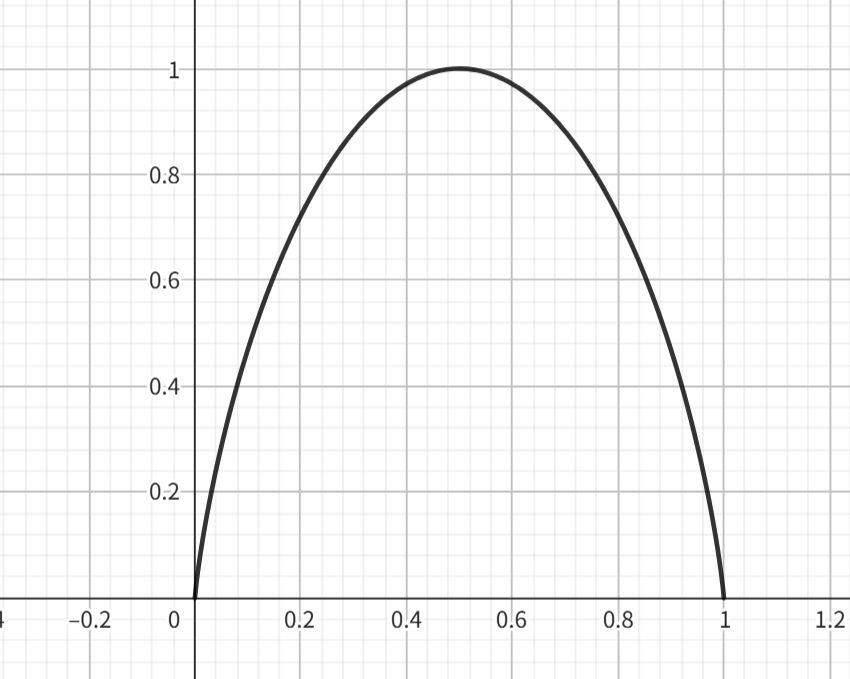
\includegraphics[width=.6\textwidth]{images/c2_1.png}
%     \caption{$H=x\log 1/x + (1-x)\log 1/(1-x)$的图像}
% \end{figure}